% !TEX encoding = UTF-8 Unicode
%%%%%%%%%%%%%%%%%%%%%%%%%%%%%%%%%%%%%%%%%
% Beamer Presentation
% LaTeX Template
% Version 1.0 (10/11/12)
%
% This template has been downloaded from:
% http://www.LaTeXTemplates.com
%
% License:
% CC BY-NC-SA 3.0 (http://creativecommons.org/licenses/by-nc-sa/3.0/)
%
%%%%%%%%%%%%%%%%%%%%%%%%%%%%%%%%%%%%%%%%%

%----------------------------------------------------------------------------------------
%	PACKAGES AND THEMES
%----------------------------------------------------------------------------------------

\documentclass{beamer}

\mode<presentation> {

% The Beamer class comes with a number of default slide themes
% which change the colors and layouts of slides. Below this is a list
% of all the themes, uncomment each in turn to see what they look like.

%\usetheme{default}
%\usetheme{AnnArbor}
%\usetheme{Antibes}
%\usetheme{Bergen}
%\usetheme{Berkeley}
%\usetheme{Berlin}
%\usetheme{Boadilla}
%\usetheme{CambridgeUS}
%\usetheme{Copenhagen}
%\usetheme{Darmstadt}
%\usetheme{Dresden}
%\usetheme{Frankfurt}
%\usetheme{Goettingen}
%\usetheme{Hannover}
%\usetheme{Ilmenau}
%\usetheme{JuanLesPins}
%\usetheme{Luebeck}
\usetheme{Madrid}
%\usetheme{Malmoe}
%\usetheme{Marburg}
%\usetheme{Montpellier}
%\usetheme{PaloAlto}
%\usetheme{Pittsburgh}
%\usetheme{Rochester}
%\usetheme{Singapore}
%\usetheme{Szeged}
%\usetheme{Warsaw}

% As well as themes, the Beamer class has a number of color themes
% for any slide theme. Uncomment each of these in turn to see how it
% changes the colors of your current slide theme.

%\usecolortheme{albatross}
%\usecolortheme{beaver}
%\usecolortheme{beetle}
%\usecolortheme{crane}
%\usecolortheme{dolphin}
%\usecolortheme{dove}
%\usecolortheme{fly}
%\usecolortheme{lily}
%\usecolortheme{orchid}
%\usecolortheme{rose}
%\usecolortheme{seagull}
%\usecolortheme{seahorse}
%\usecolortheme{whale}
%\usecolortheme{wolverine}

%\setbeamertemplate{footline} % To remove the footer line in all slides uncomment this line
%\setbeamertemplate{footline}[page number] % To replace the footer line in all slides with a simple slide count uncomment this line

%\setbeamertemplate{navigation symbols}{} % To remove the navigation symbols from the bottom of all slides uncomment this line
}

\usepackage{graphicx} % Allows including images
\usepackage{booktabs} % Allows the use of \toprule, \midrule and \bottomrule in tables
\usepackage{xeCJK}
\setCJKmainfont{SourceHanSerif-Regular}
\usepackage{color}
\usepackage{listings}
\lstset{numbers=left}
\usepackage{tikz}


%----------------------------------------------------------------------------------------
%	TITLE PAGE
%----------------------------------------------------------------------------------------

\title[Pipe]{Pipe} % The short title appears at the bottom of every slide, the full title is only on the title page

\author{张海宁} % Your name
\institute[计算机科学与技术学院] % Your institution as it will appear on the bottom of every slide, may be shorthand to save space
{
贵州大学 \\ % Your institution for the title page
\medskip
\textit{hnzhang1@gzu.edu.cn} % Your email address
}
\date{\today} % Date, can be changed to a custom date

\begin{document}

\begin{frame}
\titlepage % Print the title page as the first slide
\end{frame}

\begin{frame}
\frametitle{Overview} % Table of contents slide, comment this block out to remove it
\tableofcontents % Throughout your presentation, if you choose to use \section{} and \subsection{} commands, these will automatically be printed on this slide as an overview of your presentation
\end{frame}

%----------------------------------------------------------------------------------------
%	PRESENTATION SLIDES
%----------------------------------------------------------------------------------------
\section{Pipe}
\begin{frame}
\Huge{\centerline{Pipe}}
\end{frame}
\subsection{What is a Pipe}
\begin{frame}
\Huge{\centerline{What is a Pipe}}
\end{frame}
\begin{frame}[fragile]{Pipe}
We use the term \emph{pipe} to mean connecting a data flow from one process to another. 
\begin{block}{shell command}
\begin{verbatim}
cat <<"EOF" | grep "abc"
\end{verbatim}
\center{

\begin{tikzpicture}
%\draw [thick,red,dashed,above] (0,0) rectangle (3,5) node{host A};
\node [draw,rectangle] (kbd) at(0,0){stdin};
\node [draw,rectangle] (ls) at(2,0){cat <<"EOF"};
\node [draw,rectangle,red] (piple) at(4,0){piple};
\node [draw,rectangle] (grep) at(6,0){grep "abc"};
\node [draw,rectangle] (out) at(8,0){stdout};
%\draw [thick,blue,dashed,above] (5,0) rectangle (8,5)node{host B};
%\node [draw,rectangle] (pb1) at(6.5,3){process B1};
%\node [draw,rectangle] (pb2) at(6.5,2){...};
\draw[thick,->](kbd) to[out=0,in=180] (ls);
\draw[thick,->](ls) to[out=0,in=180] (piple);
\draw[thick,->](piple) to[out=0,in=180] (grep);
\draw[thick,->](grep) to[out=0,in=180] (out);

\end{tikzpicture}
}
\end{block}
\end{frame}
%------------------------------------------------
\section{Process pipe}
\begin{frame}
\Huge{\centerline{Process pipe}}
\end{frame}
\begin{frame}[fragile]{Process pipe}
Perhaps the simplest way of passing data between two programs is with the \emph{popen} and \emph{pclose} functions. 
\begin{block}{原型}
\begin{verbatim}
#include <stdio.h>
FILE *popen(const char *command, const char *open_mode);
int pclose(FILE *stream_to_close);
\end{verbatim}
\end{block}
\end{frame}
\begin{frame}{popen}
\centerline{
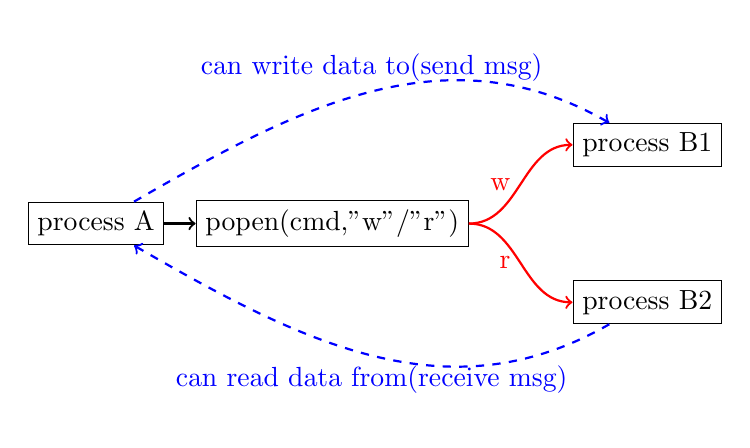
\begin{tikzpicture}
\node (A) [draw,rectangle] at(0,2) {process A};
\node (B) [draw,rectangle] at(3,2) {popen(cmd,"w"/"r")};
\draw [thick,->] (A) to[out=0,in=180](B);
\node (p1) [draw,rectangle] at(7,3) {process B1};
\node (p2) [draw,rectangle] at(7,1) {process B2};
\draw [thick,->,left,red] (B) to[out=0,in=180] node{w} (p1);
\draw [thick,->,left,red] (B) to[out=0,in=180]node{r} (p2);
\draw[thick,above,->,blue,dashed] (A) to[out=30,in=150] node{can write data to(send msg)} (p1);
\draw[thick,below,->,blue,dashed] (p2) to[out=210,in=330] node{can read data from(receive msg)} (A);
\end{tikzpicture}
}
\end{frame}

\begin{frame}[fragile]{read data from child process}
\begin{block}{12-pipeRead.c}
\begin{verbatim}
#include<unistd.h>
#include<stdio.h>
#include<stdlib.h>
#include<string.h>
int main(){
 FILE * f; char buf[1000]; int len;
 memset(buf,'\0',1000);
 f=popen("uname -a","r"); sleep(5);
 if(f==NULL){
  perror("error in create another process!"); exit(-1); }
 len = fread(buf,sizeof(char),1000,f);
 if(len>0){
  printf("the out put of uname -a is:\n%s\n",buf); }	
 printf("finished!"); pclose(f); exit(0);
}
\end{verbatim}
\end{block}
\end{frame}

\begin{frame}[fragile]{read data from child process}
\begin{block}{13-pipeRead.c}
\begin{verbatim}
./pipe &
[2] 5254
[1]   Done                    ./pipe
$ ps -j
USER           PID  PPID  PGID   SESS JOBC STAT COMMAND
hainingzhang  1583  1582  1583      0    1 S     -bash
hainingzhang  5254  1583  5254      0    1 S     ./pipe
hainingzhang  5255  5254  5254      0    1 Z    (uname)
$ the out put of uname -a is:
Darwin HainingdeMacBook-Pro.local 17.5.0 Darwin Kernel 
 Version 17.5.0: Mon Mar  5 22:24:32 PST 2018; 
  root:xnu-4570.51.1~1/RELEASE_X86_64 x86_64

finished!
\end{verbatim}
\end{block}
\end{frame}

\begin{frame}[fragile]{send data to child process}
\begin{block}{13-pipeWrite.c}
\begin{verbatim}
#include<unistd.h>
#include<stdio.h>
#include<stdlib.h>
#include<string.h>
int main(){
 FILE * f; char buf[1000]; int len;
 memset(buf,'\0',1000);
 sprintf(buf,"I can say a, b ,c and d.");		
 f=popen("wc -w","w");
 if(f==NULL){
  perror("error in create another process!");
  exit(-1); }
 fwrite(buf,sizeof(char),strlen(buf),f);
 printf("finished!"); pclose(f); exit(0);
}
\end{verbatim}
\end{block}
\end{frame}


%------------------------------------------------
%\section{Signal}
%\begin{frame}
%\Huge{\centerline{Signal}}
%\end{frame}
%------------------------------------------------
%------------------------------------------------
\begin{frame}{作业}
编写一个socket程序,要求:
\begin{enumerate}
\item
使用TCP协议实现
\item
客户端可以和服务器端进行通信
\item
当用户输入end时,本客户端退出结束
\item
进阶要求:
\begin{enumerate}
\item
多个客户端可以同时分别和服务端通信
\item
实现一个类似聊天室的功能
\end{enumerate}

\end{enumerate}
\end{frame}

\begin{frame}
\Huge{\centerline{The End}}
\end{frame}



\section{Appendix}
\begin{frame}
\Huge{\centerline{Appendix}}
\end{frame}
%----------------------------------------------------------------------------------------
\begin{frame}{本课程相关资源下载}
\begin{enumerate}
\item
ppt

\url{https://github.com/gmsft/ppt/tree/master/linux}
\item
实验指导书

\url{https://github.com/gmsft/ppt/tree/master/book/linux}
\end{enumerate}
\end{frame}
\begin{frame}
\frametitle{about man page}
The manual is generally split into eight numbered sections, organized as follows (on Research Unix, BSD, macOS and Linux):
\begin{table}
\begin{tabular}{ll}
\toprule
\textbf{section} & \textbf{description} \\
\midrule
1 & General commands\\
2 & System calls\\
3 & Library function(C standard library)\\
4 & Special files(devices) and drivers\\
5 & File formats and conventions\\
6 & Games and screensavers\\
7 & Miscellanea\\
8 & System administration commands and daemons\\  
\bottomrule
\end{tabular}
\caption{man page}
\end{table}

在终端中运行man read 与 man 2 read ,观察其输出的区别。
\end{frame}

\end{document} 
